In the following lines, a study of the location of the Ground Sations will be carried in order to know the optinal location for them. As it has been stated in the report, the study has been done using a Matlab code that can be found in [{REF TO ANNEX VI. Section 14}].

The code evaluates the visibility of a ground stations over time. For a given time, it computes the number of satellites that it has in sight. This analysis is done for a significant period of time in invertavals of a fixed time step.

\subsection{Latitude analysis}
Is easy to see that the effect of changing the latitude is practically independent for the longitude. For this reason, the links during the day for a given longitude are studied independently of the latitude and viceversa. Doing the analysis for latitudes between 0º and 90º during 2 days, with 5 minutes time-step, this are the results:
\begin{figure}[H]
\begin{center}
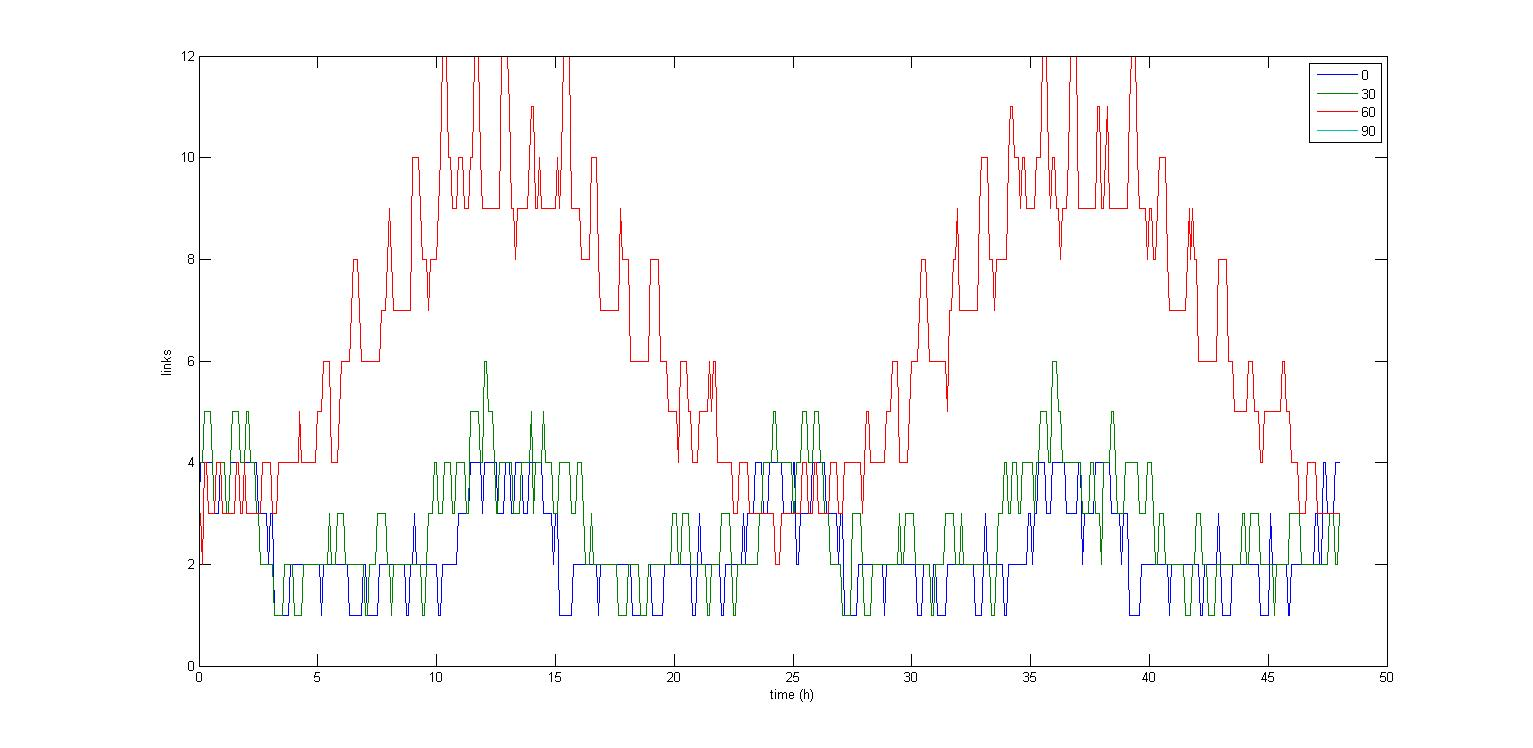
\includegraphics[scale=0.30]{0_30_90_lat.jpg}
\caption[Links vs time for latitudes from 0º to 90º]{Number of links versus time for latitudes from 0º to 90º with a time interval of 5 minutes. Dark blue line shows the results for latitude 0º, green line for 30º, red line for 60º and light blue line for 90º}
\label{fig:lat1}
\end{center}
\end{figure}
As is shown in Figure \ref{fig:lat1}, the behaviour is not constant during the day. For every day there is a peak and a valley. This is produced for the cylindrical asymmetry of the constellation. It can also be seen that the pole is not covered. This fact was considered and assumed at the design of the constellation since it doesn't involve any problem at the performance of the system. It can also be seen that for an equatorial latitude there is always 1 link, at least. The equator is the most critical place because is where satellites from different planes are more separated. Global coverage can be ensured, but is important to appreciate that for higher latitudes the coverage is better.

Doing the same analysis but for negative latitudes, the following results are obtained:
\begin{figure}[H]
\begin{center}
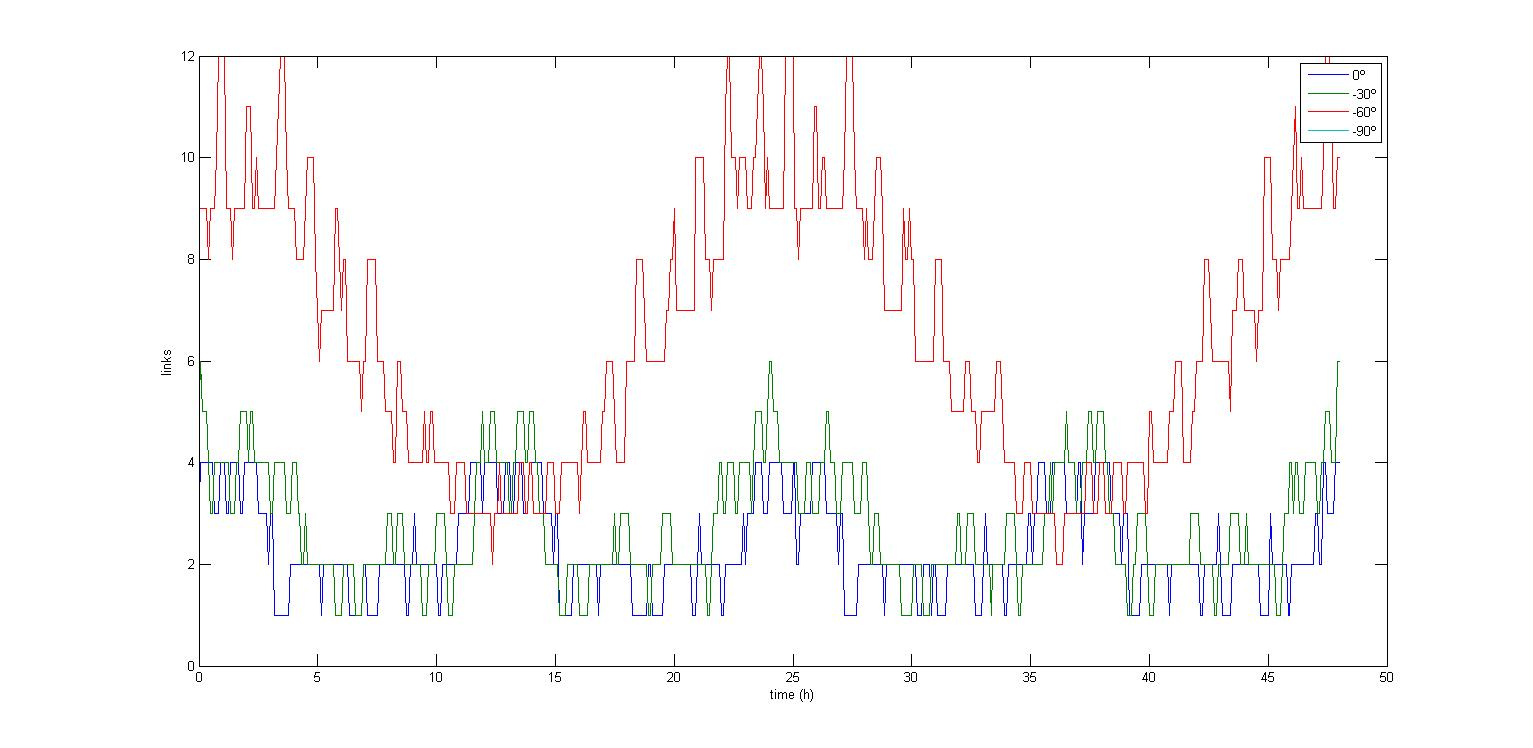
\includegraphics[scale=0.30]{0_-30_-90_lat.jpg}
\caption[Links vs time for latitudes from 0º to -90º]{Number of links versus time for latitudes from 0º to 90º with a time interval of 5 minutes. Dark blue line shows the results for latitude 0º, green line for -30º, red line for -60º and light blue line for -90º}
\label{fig:lat2}
\end{center}
\end{figure}
Comparing the results of Figure \ref{fig:lat2} with the ones of Figure \ref{fig:lat1} it is seen that they are practically the same but with an offset of 12 hours. They are also seen small local deviations, but these are not much significant because of the time-step. This time-step is of 5 minutes for a first sight of the tendencies, and it do not allow extremely precise results.

Taking into account that the results of positive latitudes can be extrapolated to negative ones, the rest of the analysis will be done only for positive latitudes.Is important to know at which latitude, close to the poles, the coverage is lost due to the geometry of the constellation.
\begin{figure}[H]
\begin{center}
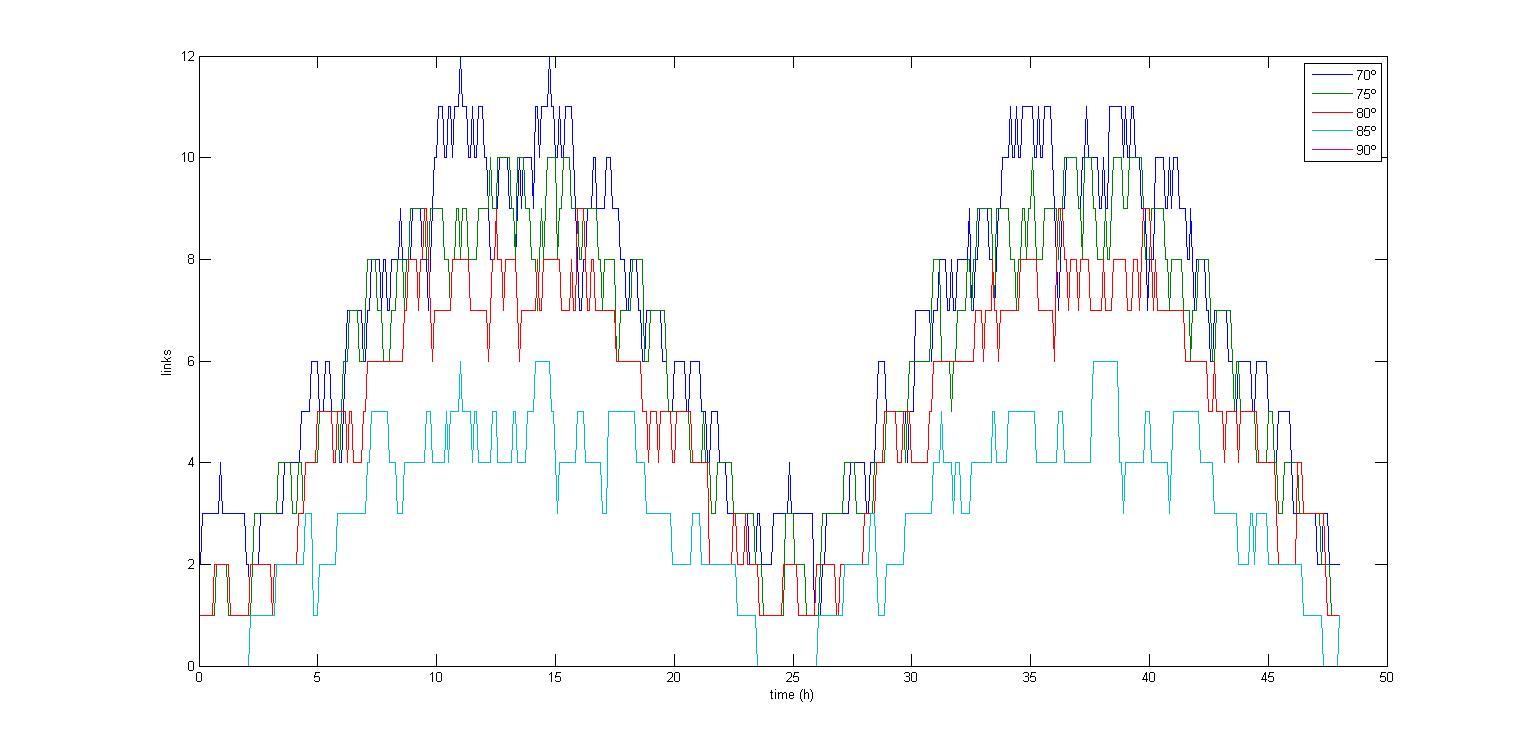
\includegraphics[scale=0.30]{70_5_90_lat.jpg}
\caption[Links vs time for latitudes from 70º to 90º]{Number of links versus time for latitudes from 70º to 90º with a time interval of 5 minutes. Dark blue line shows the results for latitude 70º, green line for 75º, red line for 80º, light blue line for 85º and violet line for 90º}
\label{fig:lat3}
\end{center}
\end{figure}
It is seen that over 80º of latitude the system starts to lose coverage. It does not cause any problem because there are not inhabited zones over +80º or under -80º. For situating the Ground Stations it has to be considered this restriction.

Now, the latitudes that can provide more links are, around 60º:
\begin{figure}[H]
\begin{center}
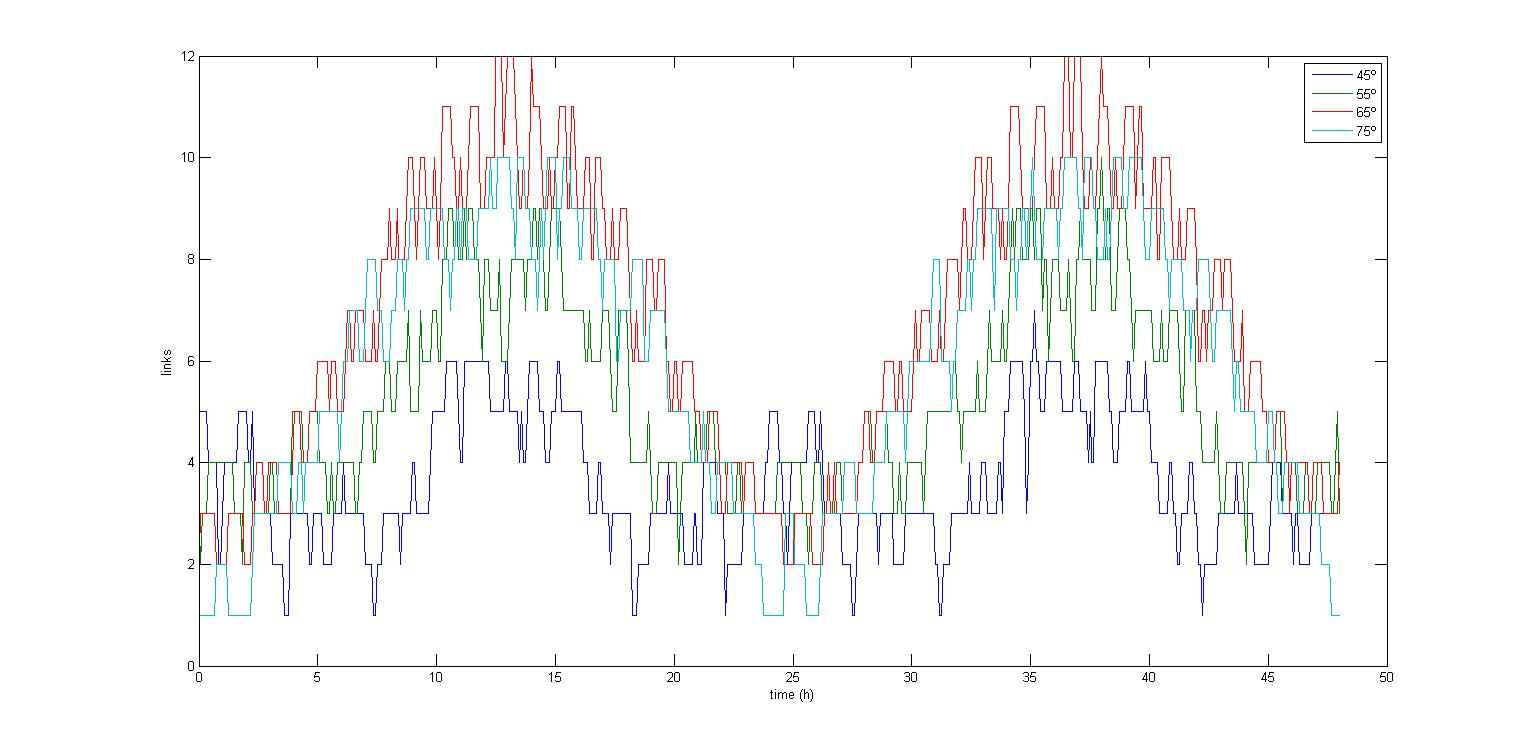
\includegraphics[scale=0.30]{45_10_75_lat.jpg}
\caption[Links vs time for latitudes from 45º to 75º]{Number of links versus time for latitudes from 45º to 75º with a time interval of 5 minutes. Dark blue line shows the results for latitude 45º, green line for 55º, red line for 65º and light blue line for 75º}
\label{fig:lat4}
\end{center}
\end{figure}
As it can be seen in Figure \ref{fig:lat4}, the optimal latitude must be between 55º and 75º. Expanding the analysis:
\begin{figure}[H]
\begin{center}
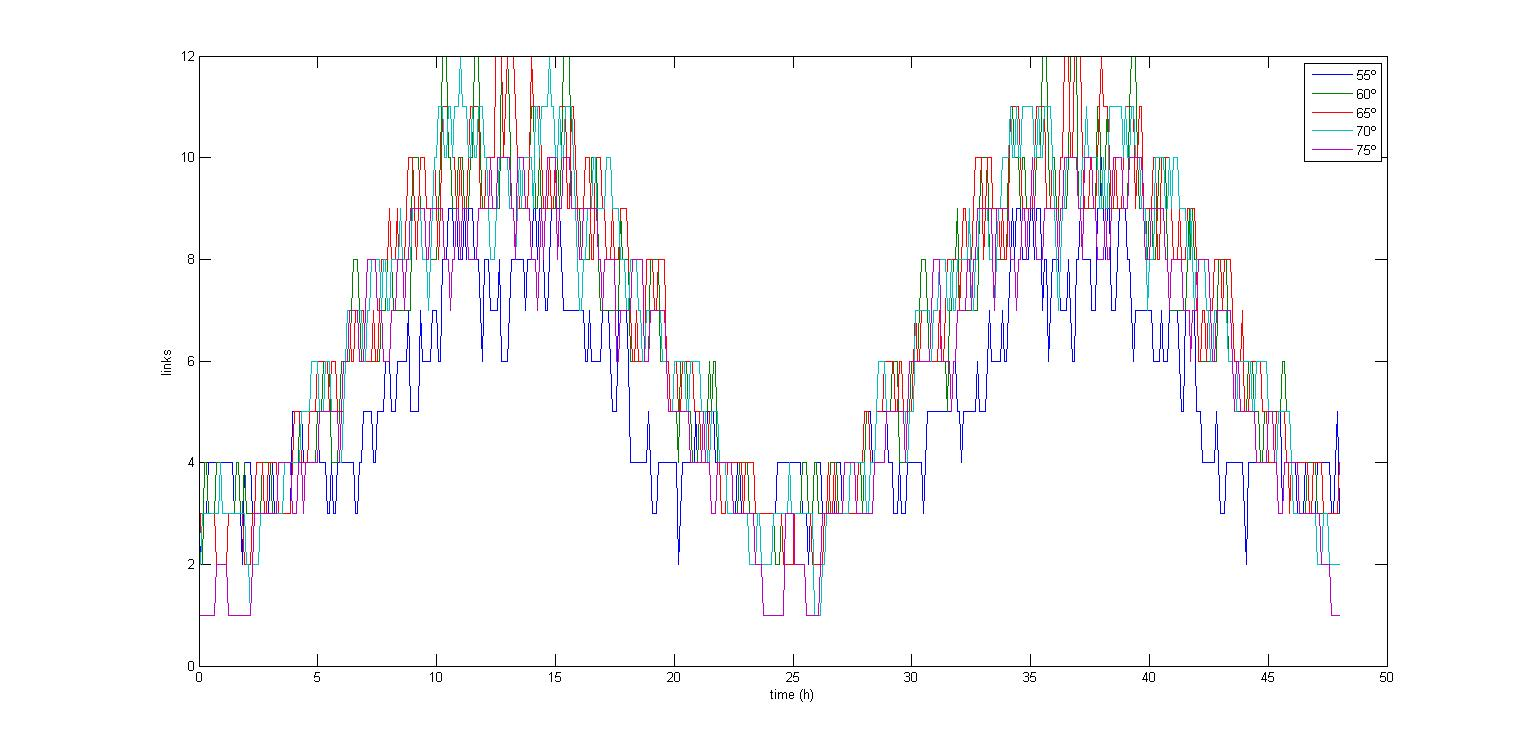
\includegraphics[scale=0.30]{55_5_75_lat.jpg}
\caption[Links vs time for latitudes from 55º to 75º]{Number of links versus time for latitudes from 55º to 75º with a time interval of 5 minutes. Dark blue line shows the results for latitude 55º, green line for 60º, red line for 65º, light blue line for 70º and violet line for 75º}
\label{fig:lat5}
\end{center}
\end{figure}
The better performance is registered around 60º and 65º. Figure \ref{fig:lat5} suggest that between 50º and 60º there is always at least 1 link. But looking it carefully, at the hour 37, there is a local deviation to 0 links. This requires a more accurate analysis decreasing the time-step. For 30 seconds time-step:
\begin{figure}[H]
\begin{center}
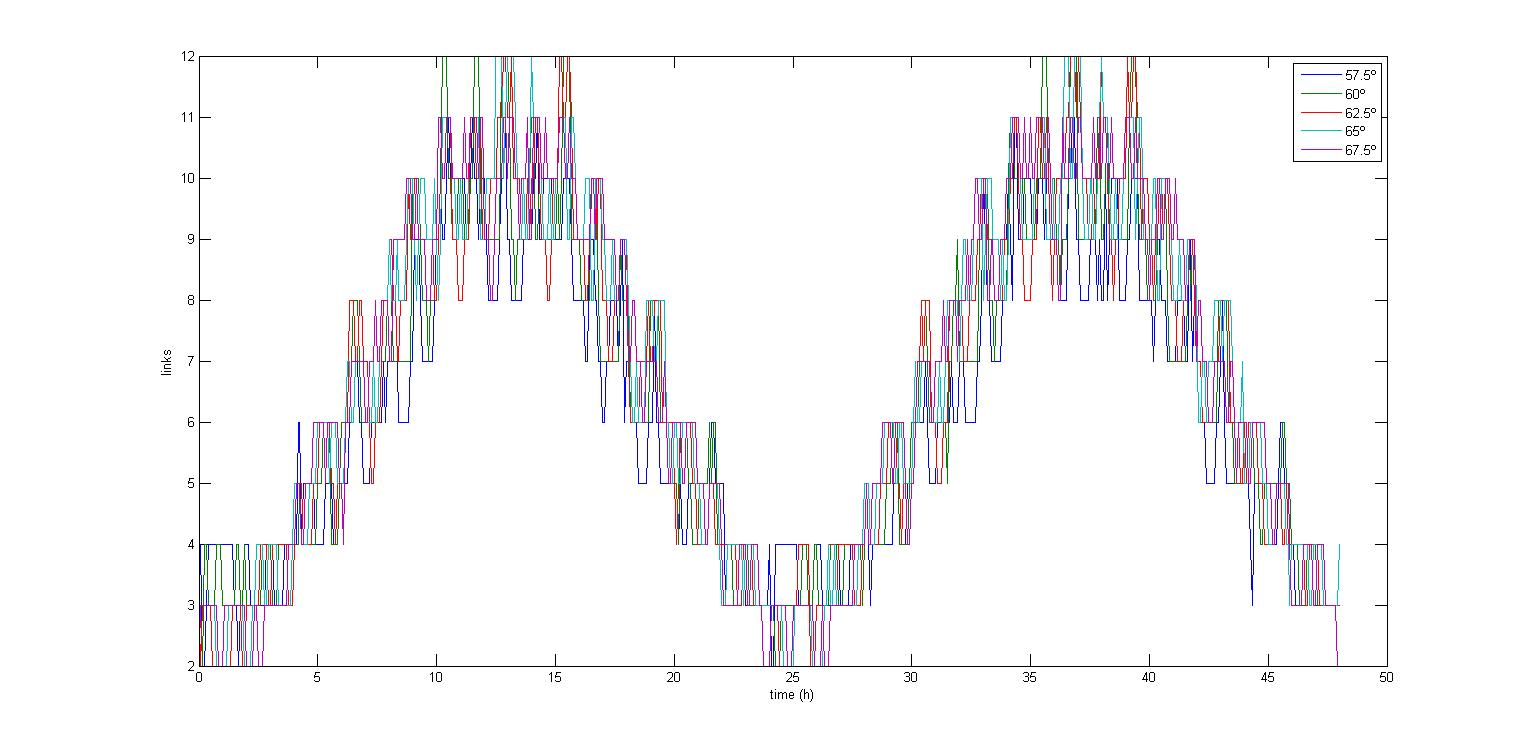
\includegraphics[scale=0.30]{575_25_675_lat.jpg}
\caption[Links vs time for latitudes from 57.5º to 67.5º]{Number of links versus time for latitudes from 57.5º to 67.5º with a time interval of 5 minutes. Dark blue line shows the results for latitude 57.5º, green line for 60º, red line for 62.5º, light blue line for 65º and violet line for 67.5º}
\label{fig:lat6}
\end{center}
\end{figure}
In Figure \ref{fig:lat6} there is no problem with the coverage. For ensuring the results and to avoid possible loses of links locally in time, the same ragne of latitudes is analyze with a smaller time-step.
\begin{figure}[H]
\begin{center}
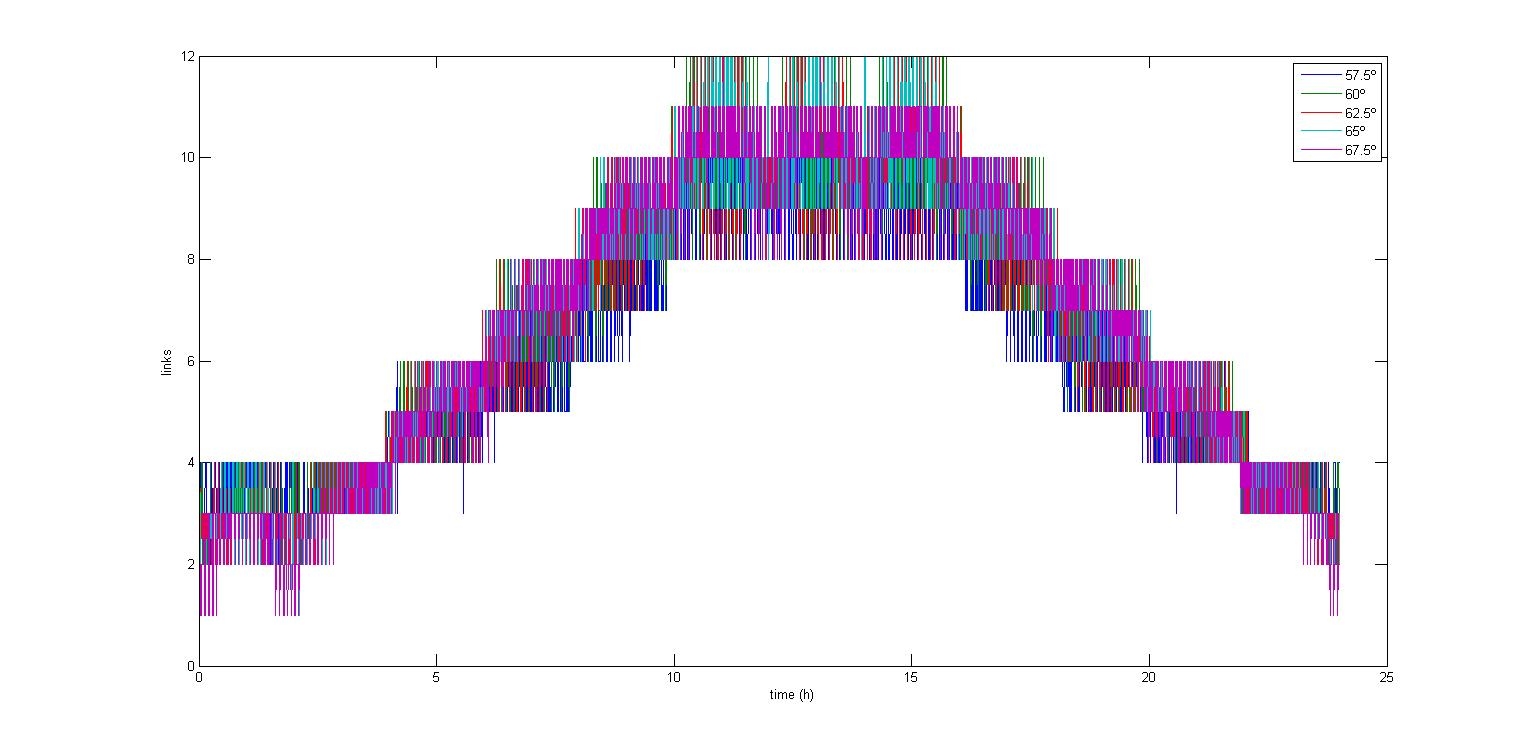
\includegraphics[scale=0.30]{575_25_675_(30s)_lat.jpg}
\caption[Links vs time for latitudes from 57.5º to 67.5º reduced timestep]{Number of links versus time for latitudes from 57.5º to 67.5º with a time interval of 30 seconds. Dark blue line shows the results for latitude 57.5º, green line for 60º, red line for 62.5º, light blue line for 65º and violet line for 67.5º}
\label{fig:lat7}
\end{center}
\end{figure}
It can be seen that between 65º and 67.5º the system loses the 2nd link and for a wile the station would be connected only to 1 satellite. It is optimum to place the stations between +57.5º and +62.5º of latitude. In order to verify the results for the opposite latitudes:
\begin{figure}[H]
\begin{center}
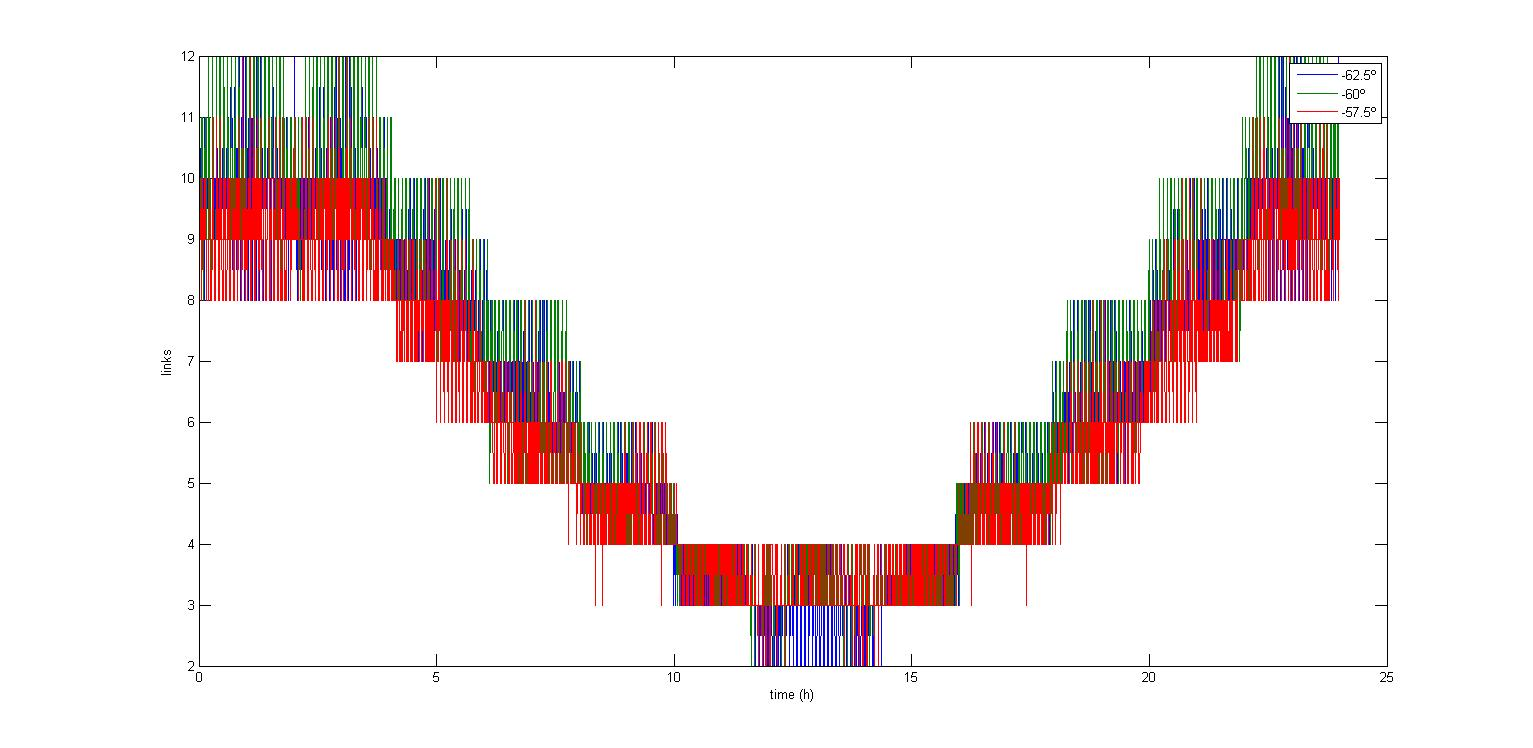
\includegraphics[scale=0.30]{-625_-25_575_(30s)_lat.jpg}
\caption[Links vs time for latitudes from -62.5º to -57.5º reduced timestep]{Number of links versus time for latitudes from -62.5º to -57.5º with a time interval of 30 seconds. Dark blue line shows the results for latitude -62.5º, green line for -60º and red line for -57.5º}
\label{fig:lat8}
\end{center}
\end{figure}
In conclusion, the optimum latitudes for the Ground Station are:
\begin{itemize}
\item Between -62.5º and -57.5º
\item Between +57.5º and +62.5º
\end{itemize}

\subsection{Longitude analysis}
It is intuitive to think that the effect of changing the longitude is delaying the evolution of the coverage. This effect is verified by the algorithm:
\begin{figure}[H]
\begin{center}
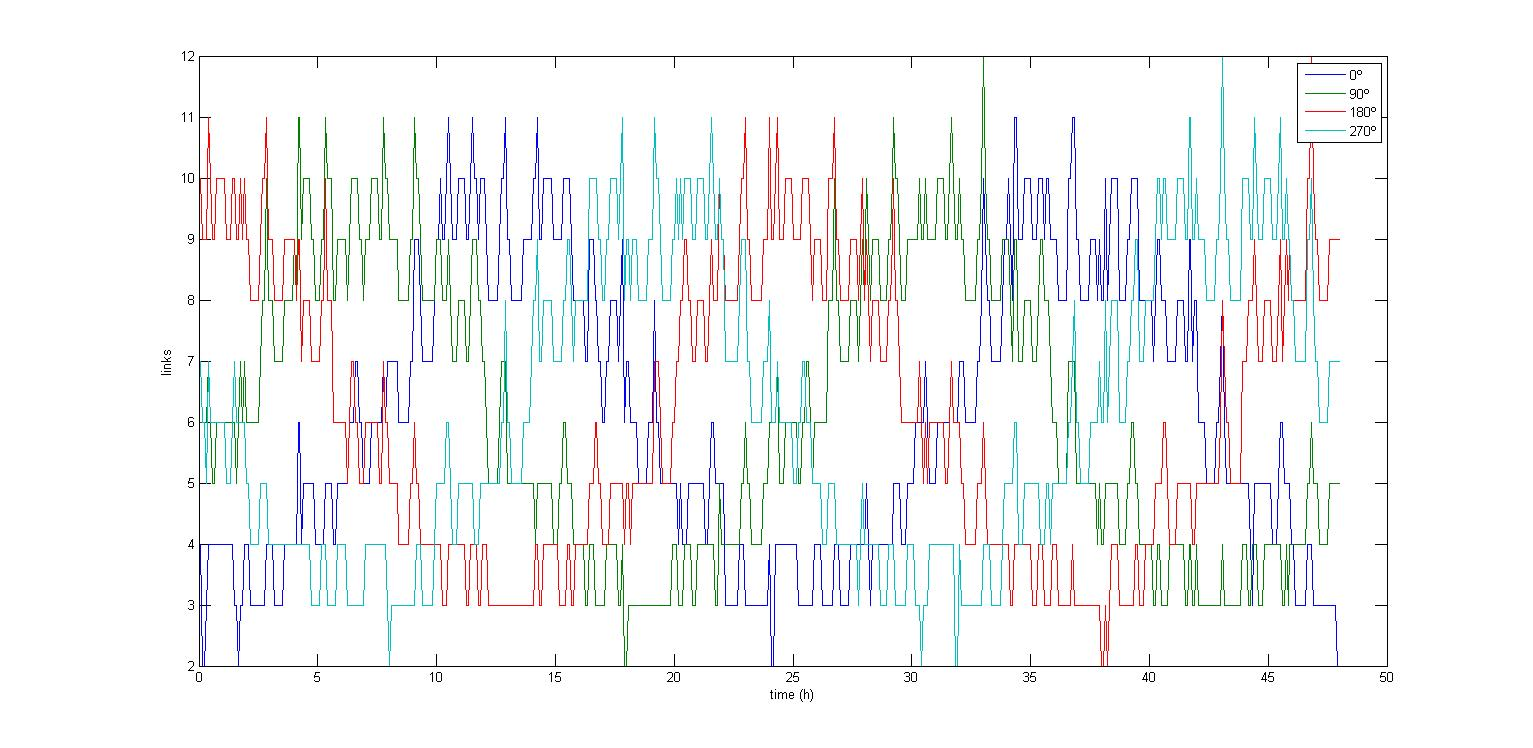
\includegraphics[scale=0.30]{0_90_270_long.jpg}
\caption{Links vs time for longitudes from 0º to 270º}
\caption[Links vs time for longitudes from 0º to 270º]{Number of links versus time for longitudes from 0º to 270º with a time interval of 5 minutes. Dark blue line shows the results for longitude 0º, green line for 90º, red line for 180º and light blue line for 270º}
\label{fig:long1}
\end{center}
\end{figure}
As it is seen in Figure \ref{fig:long1} the delay has a reason of 3 hours for every 45º of longitude. This effect can be used in order to optimize the performance of the Ground Stations. During the day every station will have a peak and a valley in the coverage. Placing the stations with a relative longitude of 120º would ensure that when one is at the valley another one is at the peak:
\begin{figure}[H]
\begin{center}
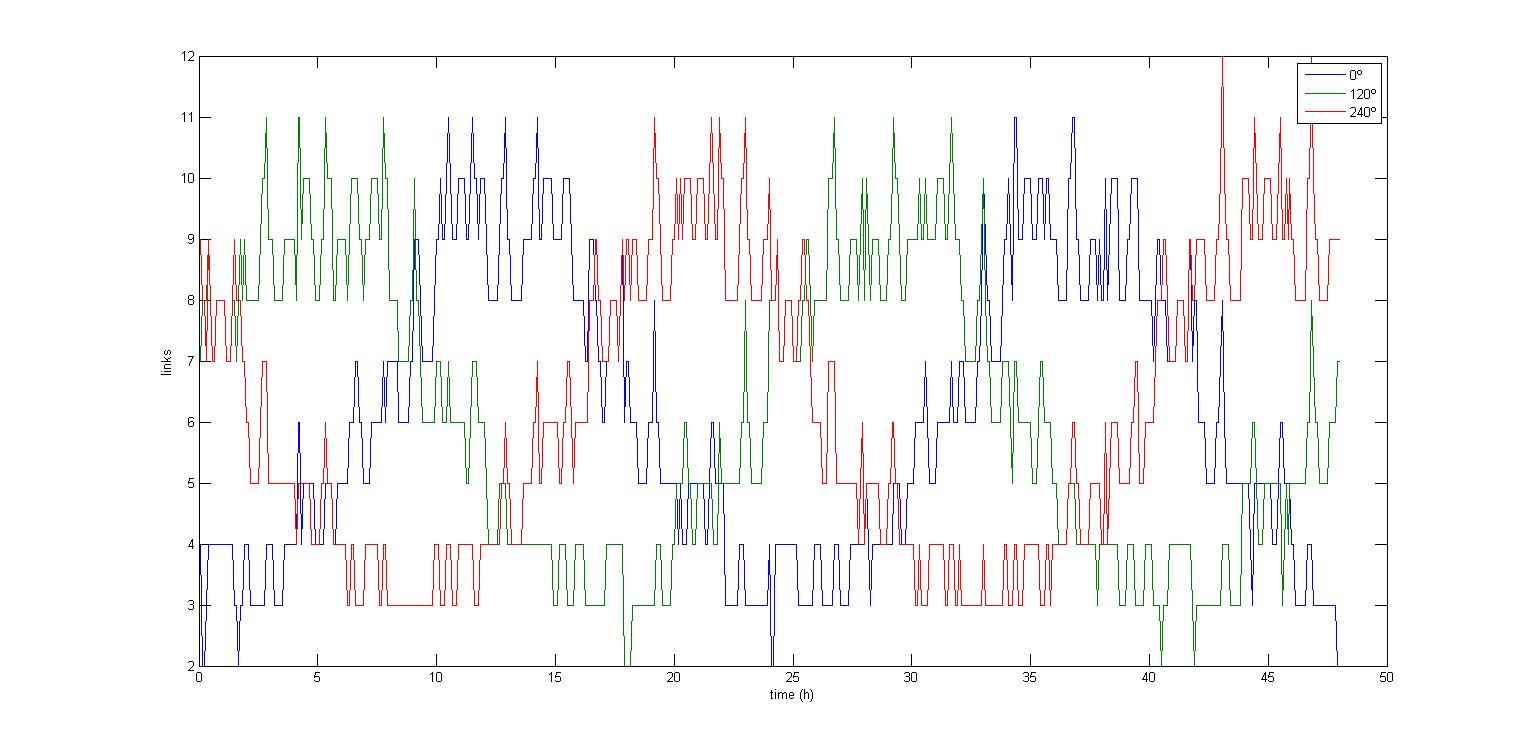
\includegraphics[scale=0.30]{0_120_240_long.jpg}
\caption[Links vs time for longitudes from 0º to 240º]{Number of links versus time for longitudes from 0º to 240º with a time interval of 5 minutes. Dark blue line shows the results for longitude 0º, green line for 120º and red line for 240º}
\label{fig:long2}
\end{center}
\end{figure}
In conclusion, the Ground Stations should be separated 120º longitude between them. It has to be taken into account that this analysis is done for stations at the same latitude. A Ground Station in a given latitude has the same coverage behaviour as an other one at the opposite latitude and 180º of longitude away. To exemplify, in the following table coordinates of equivalent places from the Ground Station point of view are showed. 
\begin{table}[H]
\begin{center}
\begin{tabular}{|c|c|c|c|c|c|c|}
\hline 
 & \multicolumn{2}{c|}{GS1} & \multicolumn{2}{c|}{GS2} & \multicolumn{2}{c|}{GS3} \\ 
\hline 
 & Latitude & Longitude & Latitude & Longitude & Latitude & Longitude \\ 
\hline 
Option 1 & 55 & 0 & 55 & 120 & 55 & 240 \\ 
\hline 
Option 2 & -55 & 180 & 55 & 120 & 55 & 240 \\ 
\hline 
Option 3 & 55 & 0 & -55 & 300 & 55 & 240 \\ 
\hline 
Option 4 & 55 & 0 & 55 & 120 & -55 & 60 \\ 
\hline 
Option 5 & -55 & 180 & -55 & 300 & 55 & 240 \\ 
\hline 
Option 6 & -55 & 180 & 55 & 120 & -55 & 60 \\ 
\hline 
Option 7 & 55 & 0 & -55 & 300 & -55 & 60 \\ 
\hline 
Option 8 & -55 & 180 & -55 & 300 & -55 & 60 \\ 
\hline 
\end{tabular}
\caption{Equivalent coordenates}
\end{center}
\end{table}